\documentclass[tikz]{standalone}
% To convert from pdf to png use the following :
%
% C:\cygwin64\bin\convert.exe -density 600 importer.pdf -resize 360x360 importer.png
%

\usepackage{listings}

\usetikzlibrary{positioning}
\usetikzlibrary{calc}
\usetikzlibrary{backgrounds}

\begin{document}
%
% Importer : Importer
%
% Note : The finder returns a \lstinline|ModuleSpec| in python 3.4 and onwards.
%
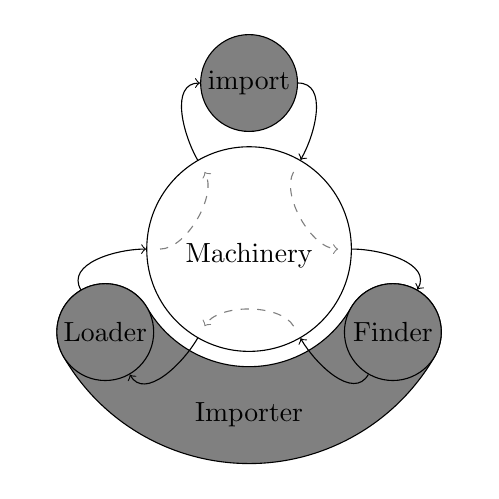
\begin{tikzpicture}
% Bounding Box
\path[use as bounding box] (-8em,-8em) rectangle (8em,8em);
% \draw circle (8em);
% Center
\coordinate (ctr) {}; % Used as an anchor for later nodes
% Import Mechanism
\node (imp) at ($(ctr) + ( 90:6em)$) [circle, draw, fill=gray, inner sep = 0.1 em, minimum size=3.5 em] {\lstinline|import|};
\node (fdr) at ($(ctr) + (-30:6em)$) [circle, draw, fill=gray, inner sep = 0.1 em, minimum size=3.5 em] {\lstinline|Finder|};
\node (ldr) at ($(ctr) + (210:6em)$) [circle, draw, fill=gray, inner sep = 0.1 em, minimum size=3.5 em] {\lstinline|Loader|};
\node (int) at (ctr)                 [circle, draw,            inner sep =   1 em, align=center] {\\ Machinery};
% Internal Structure
\draw[->, shorten >=0.5em, shorten <=0.5em, gray, dashed]  (int.60) to [out = 240, in = 180]   (int.0);
\draw[->, shorten >=0.5em, shorten <=0.5em, gray, dashed] (int.180) to [out =   0, in = -60] (int.120);
\draw[->, shorten >=0.5em, shorten <=0.5em, gray, dashed] (int.300) to [out = 120, in =  60] (int.240);
% External Structure   
\draw[->] (int) to [in =  60, out =   0] (fdr);
\draw[->] (fdr) to [in = 300, out = 240] (int);
\draw[->] (int) to [in = 180, out = 120] (imp);
\draw[->] (imp) to [in =  60, out =   0] (int);
\draw[->] (int) to [in = 300, out = 240] (ldr);
\draw[->] (ldr) to [in = 180, out = 120] (int);
% Importer
\node (Imp) at ($(ctr) + (270:6em)$)                                 {\lstinline|Importer|};
\begin{scope}[on background layer]
\draw[fill = gray] let \n{radius}={1.75em} in 
  ($(ldr) + ( 30:\n{radius})$) 
   arc( 30:210:\n{radius})     % -- ($(ldr) + (210:\n{radius})$)
   arc(210:330:6em+\n{radius}) % -- ($(fdr) + (-30:\n{radius})$)
   arc(-30:150:\n{radius})     % -- ($(fdr) + (150:\n{radius})$)
   arc(330:210:6em-\n{radius}) -- cycle;
\end{scope}
\end{tikzpicture}
\end{document}